% Options for packages loaded elsewhere
\PassOptionsToPackage{unicode}{hyperref}
\PassOptionsToPackage{hyphens}{url}
%
\documentclass[
]{article}
\usepackage{amsmath,amssymb}
\usepackage{lmodern}
\usepackage{iftex}
\ifPDFTeX
  \usepackage[T1]{fontenc}
  \usepackage[utf8]{inputenc}
  \usepackage{textcomp} % provide euro and other symbols
\else % if luatex or xetex
  \usepackage{unicode-math}
  \defaultfontfeatures{Scale=MatchLowercase}
  \defaultfontfeatures[\rmfamily]{Ligatures=TeX,Scale=1}
\fi
% Use upquote if available, for straight quotes in verbatim environments
\IfFileExists{upquote.sty}{\usepackage{upquote}}{}
\IfFileExists{microtype.sty}{% use microtype if available
  \usepackage[]{microtype}
  \UseMicrotypeSet[protrusion]{basicmath} % disable protrusion for tt fonts
}{}
\makeatletter
\@ifundefined{KOMAClassName}{% if non-KOMA class
  \IfFileExists{parskip.sty}{%
    \usepackage{parskip}
  }{% else
    \setlength{\parindent}{0pt}
    \setlength{\parskip}{6pt plus 2pt minus 1pt}}
}{% if KOMA class
  \KOMAoptions{parskip=half}}
\makeatother
\usepackage{xcolor}
\usepackage[margin=1in]{geometry}
\usepackage{color}
\usepackage{fancyvrb}
\newcommand{\VerbBar}{|}
\newcommand{\VERB}{\Verb[commandchars=\\\{\}]}
\DefineVerbatimEnvironment{Highlighting}{Verbatim}{commandchars=\\\{\}}
% Add ',fontsize=\small' for more characters per line
\usepackage{framed}
\definecolor{shadecolor}{RGB}{248,248,248}
\newenvironment{Shaded}{\begin{snugshade}}{\end{snugshade}}
\newcommand{\AlertTok}[1]{\textcolor[rgb]{0.94,0.16,0.16}{#1}}
\newcommand{\AnnotationTok}[1]{\textcolor[rgb]{0.56,0.35,0.01}{\textbf{\textit{#1}}}}
\newcommand{\AttributeTok}[1]{\textcolor[rgb]{0.77,0.63,0.00}{#1}}
\newcommand{\BaseNTok}[1]{\textcolor[rgb]{0.00,0.00,0.81}{#1}}
\newcommand{\BuiltInTok}[1]{#1}
\newcommand{\CharTok}[1]{\textcolor[rgb]{0.31,0.60,0.02}{#1}}
\newcommand{\CommentTok}[1]{\textcolor[rgb]{0.56,0.35,0.01}{\textit{#1}}}
\newcommand{\CommentVarTok}[1]{\textcolor[rgb]{0.56,0.35,0.01}{\textbf{\textit{#1}}}}
\newcommand{\ConstantTok}[1]{\textcolor[rgb]{0.00,0.00,0.00}{#1}}
\newcommand{\ControlFlowTok}[1]{\textcolor[rgb]{0.13,0.29,0.53}{\textbf{#1}}}
\newcommand{\DataTypeTok}[1]{\textcolor[rgb]{0.13,0.29,0.53}{#1}}
\newcommand{\DecValTok}[1]{\textcolor[rgb]{0.00,0.00,0.81}{#1}}
\newcommand{\DocumentationTok}[1]{\textcolor[rgb]{0.56,0.35,0.01}{\textbf{\textit{#1}}}}
\newcommand{\ErrorTok}[1]{\textcolor[rgb]{0.64,0.00,0.00}{\textbf{#1}}}
\newcommand{\ExtensionTok}[1]{#1}
\newcommand{\FloatTok}[1]{\textcolor[rgb]{0.00,0.00,0.81}{#1}}
\newcommand{\FunctionTok}[1]{\textcolor[rgb]{0.00,0.00,0.00}{#1}}
\newcommand{\ImportTok}[1]{#1}
\newcommand{\InformationTok}[1]{\textcolor[rgb]{0.56,0.35,0.01}{\textbf{\textit{#1}}}}
\newcommand{\KeywordTok}[1]{\textcolor[rgb]{0.13,0.29,0.53}{\textbf{#1}}}
\newcommand{\NormalTok}[1]{#1}
\newcommand{\OperatorTok}[1]{\textcolor[rgb]{0.81,0.36,0.00}{\textbf{#1}}}
\newcommand{\OtherTok}[1]{\textcolor[rgb]{0.56,0.35,0.01}{#1}}
\newcommand{\PreprocessorTok}[1]{\textcolor[rgb]{0.56,0.35,0.01}{\textit{#1}}}
\newcommand{\RegionMarkerTok}[1]{#1}
\newcommand{\SpecialCharTok}[1]{\textcolor[rgb]{0.00,0.00,0.00}{#1}}
\newcommand{\SpecialStringTok}[1]{\textcolor[rgb]{0.31,0.60,0.02}{#1}}
\newcommand{\StringTok}[1]{\textcolor[rgb]{0.31,0.60,0.02}{#1}}
\newcommand{\VariableTok}[1]{\textcolor[rgb]{0.00,0.00,0.00}{#1}}
\newcommand{\VerbatimStringTok}[1]{\textcolor[rgb]{0.31,0.60,0.02}{#1}}
\newcommand{\WarningTok}[1]{\textcolor[rgb]{0.56,0.35,0.01}{\textbf{\textit{#1}}}}
\usepackage{longtable,booktabs,array}
\usepackage{calc} % for calculating minipage widths
% Correct order of tables after \paragraph or \subparagraph
\usepackage{etoolbox}
\makeatletter
\patchcmd\longtable{\par}{\if@noskipsec\mbox{}\fi\par}{}{}
\makeatother
% Allow footnotes in longtable head/foot
\IfFileExists{footnotehyper.sty}{\usepackage{footnotehyper}}{\usepackage{footnote}}
\makesavenoteenv{longtable}
\usepackage{graphicx}
\makeatletter
\def\maxwidth{\ifdim\Gin@nat@width>\linewidth\linewidth\else\Gin@nat@width\fi}
\def\maxheight{\ifdim\Gin@nat@height>\textheight\textheight\else\Gin@nat@height\fi}
\makeatother
% Scale images if necessary, so that they will not overflow the page
% margins by default, and it is still possible to overwrite the defaults
% using explicit options in \includegraphics[width, height, ...]{}
\setkeys{Gin}{width=\maxwidth,height=\maxheight,keepaspectratio}
% Set default figure placement to htbp
\makeatletter
\def\fps@figure{htbp}
\makeatother
\setlength{\emergencystretch}{3em} % prevent overfull lines
\providecommand{\tightlist}{%
  \setlength{\itemsep}{0pt}\setlength{\parskip}{0pt}}
\setcounter{secnumdepth}{-\maxdimen} % remove section numbering
\ifLuaTeX
\usepackage[bidi=basic]{babel}
\else
\usepackage[bidi=default]{babel}
\fi
% get rid of language-specific shorthands (see #6817):
\let\LanguageShortHands\languageshorthands
\def\languageshorthands#1{}
\ifLuaTeX
  \usepackage{selnolig}  % disable illegal ligatures
\fi
\IfFileExists{bookmark.sty}{\usepackage{bookmark}}{\usepackage{hyperref}}
\IfFileExists{xurl.sty}{\usepackage{xurl}}{} % add URL line breaks if available
\urlstyle{same} % disable monospaced font for URLs
\hypersetup{
  pdftitle={Segunda entrega},
  pdfauthor={Diego Cubides,Larry castro, Tomas Mendez y Jersson avila},
  pdflang={es.MX},
  hidelinks,
  pdfcreator={LaTeX via pandoc}}

\title{Segunda entrega}
\author{Diego Cubides,Larry castro, Tomas Mendez y Jersson avila}
\date{2023-04-21}

\begin{document}
\maketitle

{
\setcounter{tocdepth}{3}
\tableofcontents
}
\hypertarget{introducciuxf3n}{%
\subsection{Introducción}\label{introducciuxf3n}}

El presente reporte está basado en la implementación de un aprendizaje
de máquina para poder predecir tres tipos de obstáculos mediante el
algoritmo de Knn y la distancia bajo un modelo lineal y otro multilíneal
de dos sensores incorporados en un carro a control remoto. Este robot
fue implementado en Arduino y una app móvil con el fin de obtener datos
de un sensor infrarrojo y un ultrasónico a distancias y obstáculos
diferentes.

\hypertarget{materiales}{%
\subsection{Materiales}\label{materiales}}

\begin{itemize}
\tightlist
\item
  Sensor ultrasónico US-016
\item
  Sensor Infrarrojo 2Y0A21 F
\item
  Modulo puente h l298n
\item
  Carro a control remoto
\item
  bluetooth hc-05
\item
  Arduino UNO
\end{itemize}

\hypertarget{software}{%
\subsection{Software}\label{software}}

\begin{itemize}
\tightlist
\item
  RStudio
\item
  Arduino
\item
  App inventor
\item
  Excel
\item
  PLX-DAQ
\end{itemize}

\hypertarget{procedimiento}{%
\subsection{Procedimiento}\label{procedimiento}}

\hypertarget{adquisision-de-datos}{%
\section{1.1 adquisision de datos}\label{adquisision-de-datos}}

Se programo un carro a control remoto vía bluetooth capaz de moverse a
diferentes velocidades y en cualquier dirección, este fue controlado con
una app creada en app inventor la cual permitio controlar el movimiento
del carro y enviar la acción para que envié el dato censado en ese
momento.

\begin{figure}
\centering
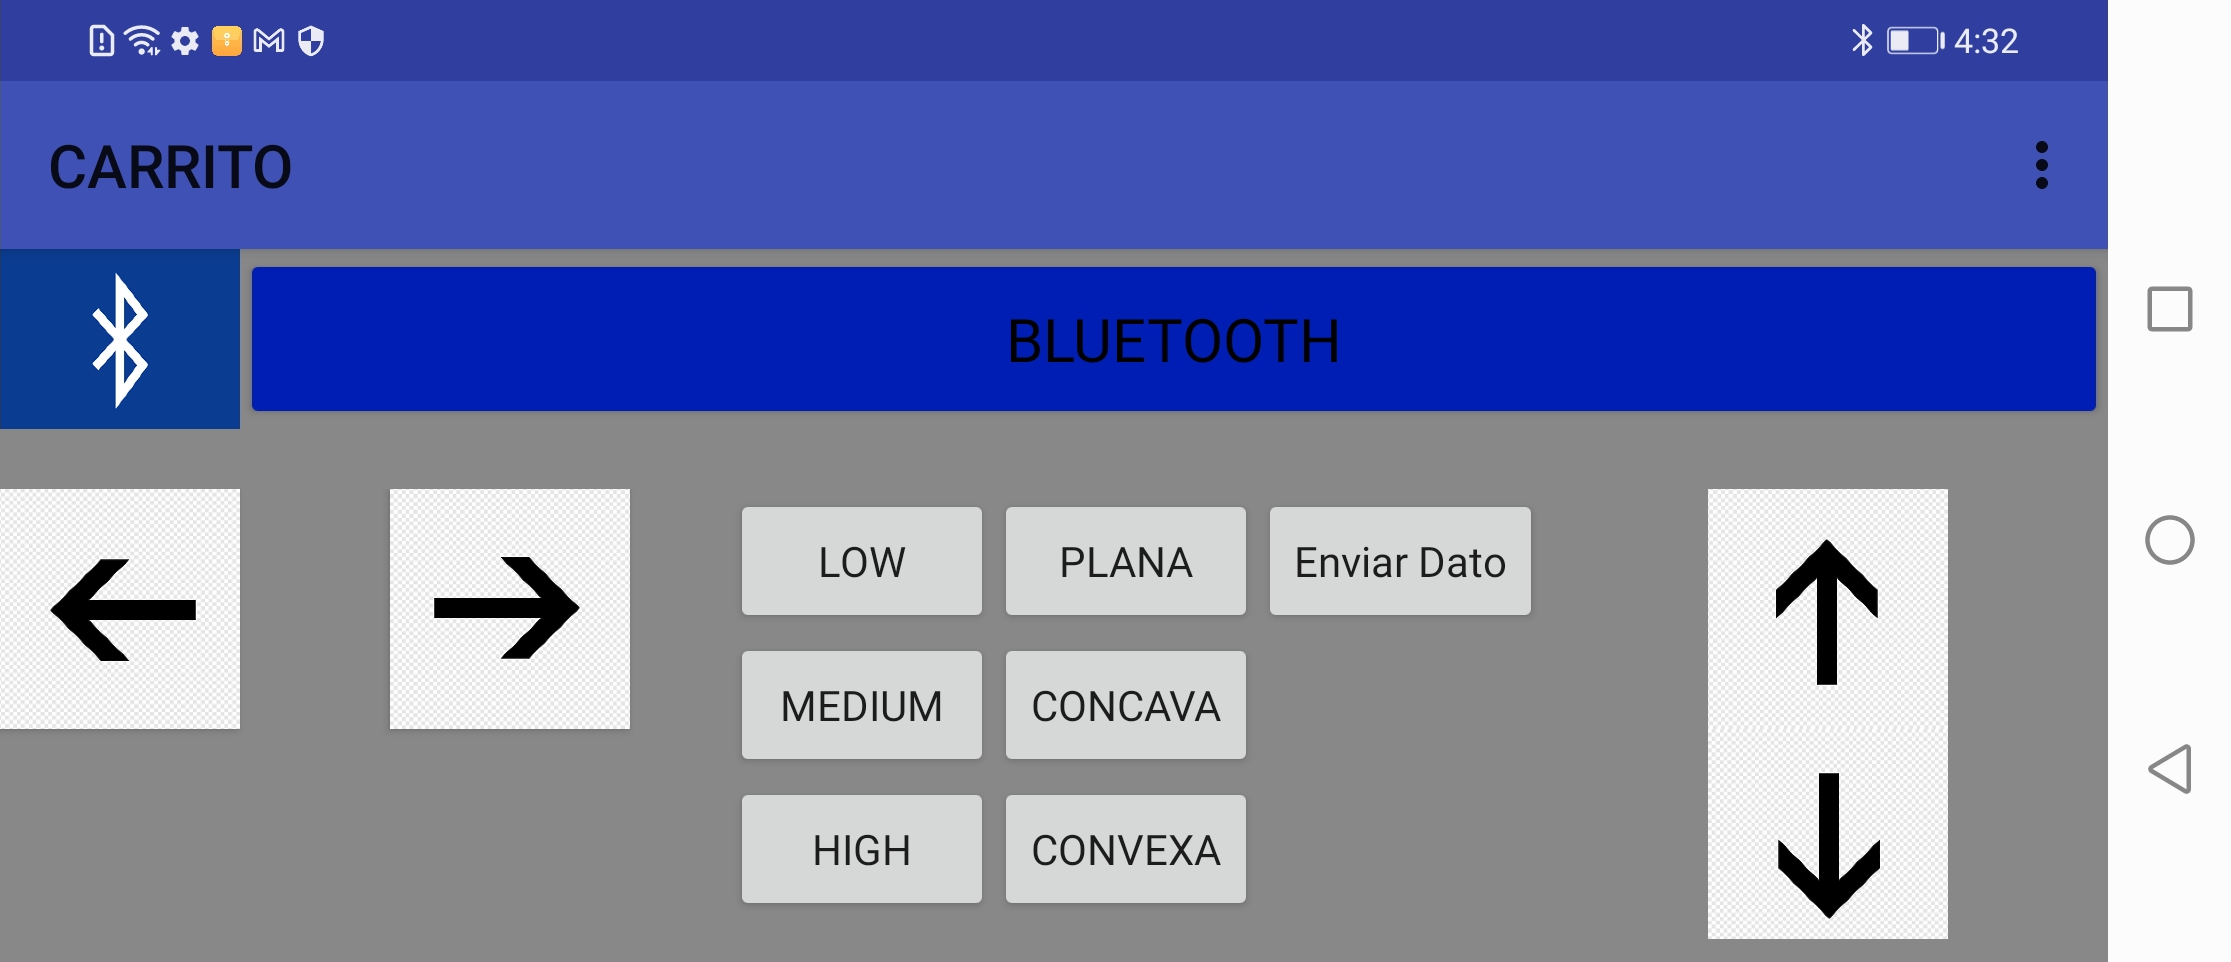
\includegraphics[width=4.91667in,height=\textheight]{app.png}
\caption{App}
\end{figure}

\begin{figure}
\centering
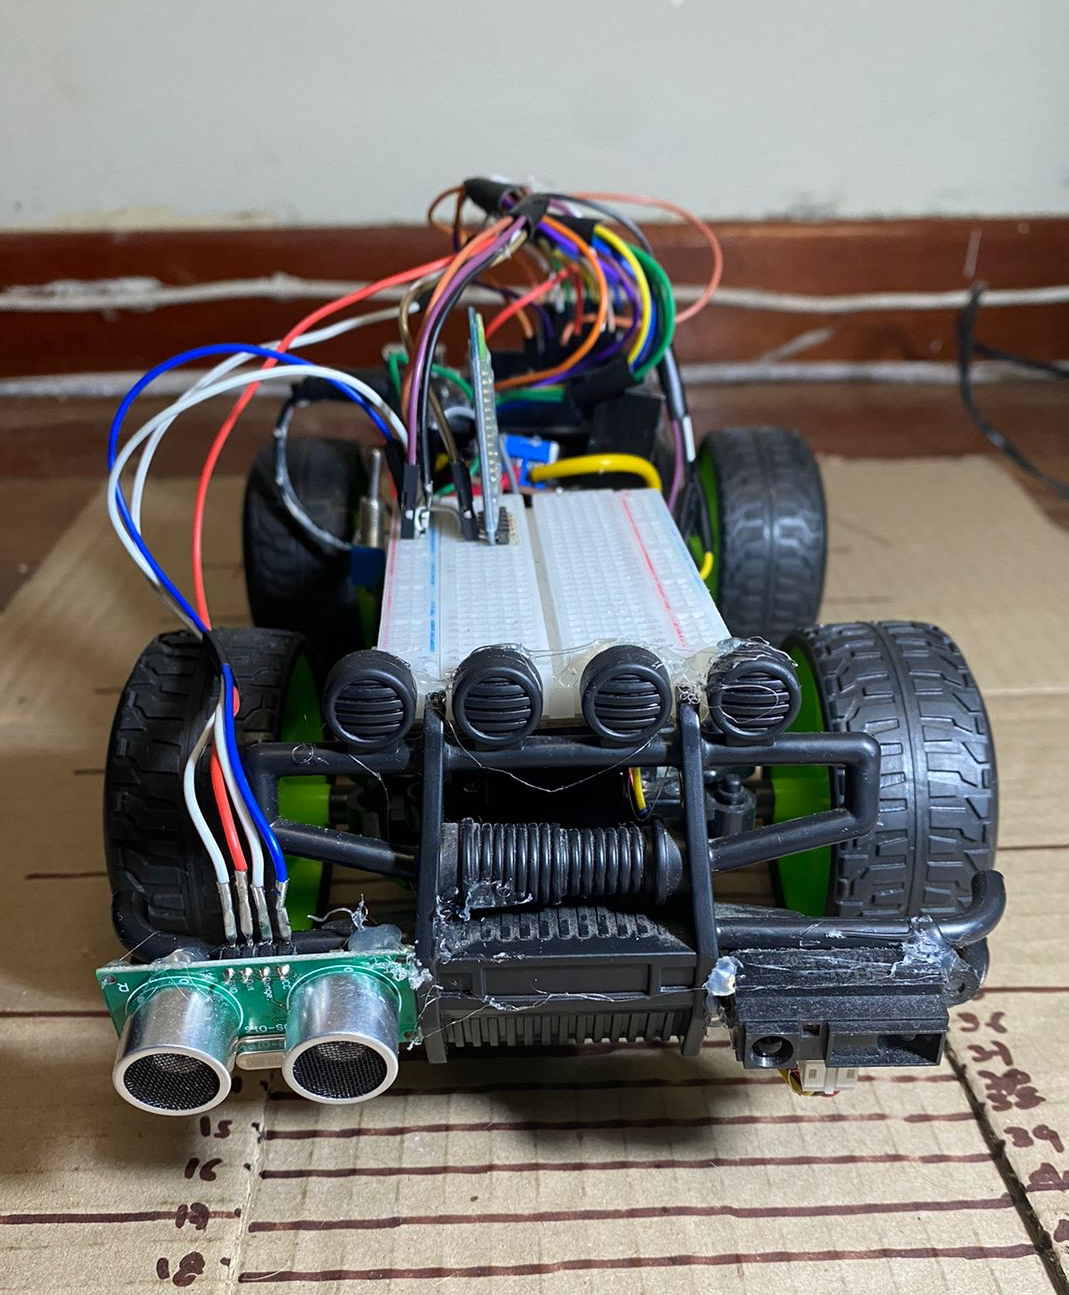
\includegraphics[width=2.96875in,height=\textheight]{carro.png}
\caption{Carro}
\end{figure}

Usando la comunicación Serial entre el Arduino y el módulo bluetooth se
pudieron captar los datos de los sensores en Excel, para poder comunicar
Excel con el Arduino se usó el software PLZ-DAQ

\begin{figure}
\centering
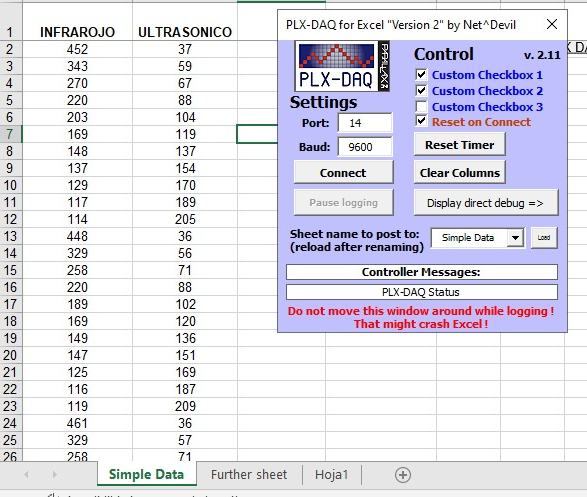
\includegraphics[width=2.30208in,height=\textheight]{plx.png}
\caption{PLX-DAQ}
\end{figure}

\hypertarget{modelo-lineal-y-regresion-multilineal}{%
\section{1.2 Modelo lineal y regresion
multilineal}\label{modelo-lineal-y-regresion-multilineal}}

Luego de tener el dataset de los datos tomados se carga la libreria
tidyverse y el dataset

\begin{Shaded}
\begin{Highlighting}[]
\FunctionTok{library}\NormalTok{(tidyverse)}
\NormalTok{folder }\OtherTok{\textless{}{-}}  \FunctionTok{dirname}\NormalTok{(rstudioapi}\SpecialCharTok{::}\FunctionTok{getSourceEditorContext}\NormalTok{()}\SpecialCharTok{$}\NormalTok{path )}
\NormalTok{wall.distance }\OtherTok{\textless{}{-}}\FunctionTok{read\_csv}\NormalTok{(}\FunctionTok{paste0}\NormalTok{(folder,}\StringTok{"/dataset\_wall\_distance.csv"}\NormalTok{))}
\end{Highlighting}
\end{Shaded}

Se hace el analisis exploratorio de datos para el dataset

\begin{Shaded}
\begin{Highlighting}[]
\FunctionTok{kable}\NormalTok{(}\FunctionTok{summary}\NormalTok{(wall.distance))}
\end{Highlighting}
\end{Shaded}

\begin{longtable}[]{@{}llll@{}}
\toprule()
& INFRARED & ULTRASONIC & DISTANCE(cm) \\
\midrule()
\endhead
& Min. :113.0 & Min. : 35.0 & Min. :10 \\
& 1st Qu.:133.8 & 1st Qu.: 71.0 & 1st Qu.:20 \\
& Median :169.0 & Median :120.0 & Median :35 \\
& Mean :207.5 & Mean :119.9 & Mean :35 \\
& 3rd Qu.:258.8 & 3rd Qu.:168.5 & 3rd Qu.:50 \\
& Max. :461.0 & Max. :209.0 & Max. :60 \\
\bottomrule()
\end{longtable}

De la tabla se puede identificar los valores maximos y minimos que se
captaron con los sensores, de igual manera los valores por el primer
quartil y el tercer cuartil

\begin{Shaded}
\begin{Highlighting}[]
\FunctionTok{hist}\NormalTok{(wall.distance}\SpecialCharTok{$}\NormalTok{INFRARED,}\AttributeTok{breaks =} \DecValTok{10}\NormalTok{)}
\end{Highlighting}
\end{Shaded}

\includegraphics{SegundaEntrega_files/figure-latex/unnamed-chunk-3-1.pdf}

\begin{Shaded}
\begin{Highlighting}[]
\FunctionTok{hist}\NormalTok{(wall.distance}\SpecialCharTok{$}\NormalTok{ULTRASONIC,}\AttributeTok{breaks =} \DecValTok{10}\NormalTok{)}
\end{Highlighting}
\end{Shaded}

\includegraphics{SegundaEntrega_files/figure-latex/unnamed-chunk-3-2.pdf}
Debido a que la variable predictora es la distancia se tiene que pasar
como factor,Graficando cada dato del sensor con la función hist se puede
ver que los datos están distribuidos y que son viables para hacer
aprendizaje de maquina

\begin{Shaded}
\begin{Highlighting}[]
\NormalTok{wall.distance2}\SpecialCharTok{$}\StringTok{\textasciigrave{}}\AttributeTok{DISTANCE(cm)}\StringTok{\textasciigrave{}} \OtherTok{\textless{}{-}}\FunctionTok{as.factor}\NormalTok{(wall.distance2}\SpecialCharTok{$}\StringTok{\textasciigrave{}}\AttributeTok{DISTANCE(cm)}\StringTok{\textasciigrave{}}\NormalTok{)}
\FunctionTok{pairs}\NormalTok{(wall.distance[}\FunctionTok{c}\NormalTok{(}\StringTok{"INFRARED"}\NormalTok{,}\StringTok{"ULTRASONIC"}\NormalTok{)]}
\NormalTok{,}\AttributeTok{pch=}\DecValTok{25}
\NormalTok{,}\AttributeTok{bg=}\FunctionTok{c}\NormalTok{(}\StringTok{"green"}\NormalTok{,}\StringTok{"blue3"}\NormalTok{,}\StringTok{"gray"}\NormalTok{,}\StringTok{"yellow"}\NormalTok{,}\StringTok{"green3"}\NormalTok{,}\StringTok{"pink"}\NormalTok{,}\StringTok{"brown"}\NormalTok{,}\StringTok{"black"}\NormalTok{,}\StringTok{"red"}\NormalTok{,}\StringTok{"orange"}\NormalTok{)[}\FunctionTok{unclass}\NormalTok{(wall.distance2}\SpecialCharTok{$}\StringTok{\textasciigrave{}}\AttributeTok{DISTANCE(cm)}\StringTok{\textasciigrave{}}\NormalTok{)])}
\end{Highlighting}
\end{Shaded}

\includegraphics{SegundaEntrega_files/figure-latex/unnamed-chunk-4-1.pdf}
Cuando se captaron los datos se identificó que un sensor crece
inversamente al otro, graficando todos los datos en función a la
distancia se notó que tienen una buena distribución y que se logran
identificar grupos en todos los datos

\begin{Shaded}
\begin{Highlighting}[]
\FunctionTok{pairs.panels}\NormalTok{(wall.distance2[}\FunctionTok{c}\NormalTok{(}\StringTok{"INFRARED"}\NormalTok{,}\StringTok{"ULTRASONIC"}\NormalTok{)]}
\NormalTok{             ,}\AttributeTok{pch=}\DecValTok{21}\NormalTok{,}\AttributeTok{bg=}\FunctionTok{c}\NormalTok{(}\StringTok{"green"}\NormalTok{,}\StringTok{"blue3"}\NormalTok{,}\StringTok{"gray"}\NormalTok{,}\StringTok{"yellow"}\NormalTok{,}\StringTok{"green3"}\NormalTok{,}\StringTok{"pink"}\NormalTok{,}\StringTok{"brown"}\NormalTok{,}\StringTok{"black"}\NormalTok{,}\StringTok{"red"}\NormalTok{,}\StringTok{"orange"}\NormalTok{)[}\FunctionTok{unclass}\NormalTok{(wall.distance2}\SpecialCharTok{$}\StringTok{\textasciigrave{}}\AttributeTok{DISTANCE(cm)}\StringTok{\textasciigrave{}}\NormalTok{)])}
\end{Highlighting}
\end{Shaded}

\includegraphics{SegundaEntrega_files/figure-latex/unnamed-chunk-5-1.pdf}
En esta grafica se ve mejor la relacion de las varibales y se ve que
tiene una relacion negativa de -0.9, siendo esto un factor muy
importante para poder hacer el aprendizaje de maquina

\begin{Shaded}
\begin{Highlighting}[]
\FunctionTok{kable}\NormalTok{(}\FunctionTok{prop.table}\NormalTok{(}\FunctionTok{table}\NormalTok{(wall.distance}\SpecialCharTok{$}\StringTok{\textasciigrave{}}\AttributeTok{DISTANCE(cm)}\StringTok{\textasciigrave{}}\NormalTok{)))}
\end{Highlighting}
\end{Shaded}

\begin{longtable}[]{@{}lr@{}}
\toprule()
Var1 & Freq \\
\midrule()
\endhead
10 & 0.0909091 \\
15 & 0.0909091 \\
20 & 0.0909091 \\
25 & 0.0909091 \\
30 & 0.0909091 \\
35 & 0.0909091 \\
40 & 0.0909091 \\
45 & 0.0909091 \\
50 & 0.0909091 \\
55 & 0.0909091 \\
60 & 0.0909091 \\
\bottomrule()
\end{longtable}

de los 110 datos que se obtuvieron hay la misma cantidad en cada
distancia identificada -regresion lineal para sensor infrarojo

\begin{Shaded}
\begin{Highlighting}[]
\NormalTok{x }\OtherTok{\textless{}{-}}\NormalTok{ dataset}\SpecialCharTok{$}\NormalTok{INFRARED}
\NormalTok{y }\OtherTok{\textless{}{-}}\NormalTok{ dataset}\SpecialCharTok{$}\StringTok{\textasciigrave{}}\AttributeTok{DISTANCE(cm)}\StringTok{\textasciigrave{}}
\NormalTok{b}\OtherTok{=}\FunctionTok{cov}\NormalTok{(x,y)}\SpecialCharTok{/}\FunctionTok{var}\NormalTok{(x)}
\NormalTok{a}\OtherTok{=}\FunctionTok{mean}\NormalTok{(y)}\SpecialCharTok{{-}}\NormalTok{b}\SpecialCharTok{*}\FunctionTok{mean}\NormalTok{(x)}
\NormalTok{a}\SpecialCharTok{+}\NormalTok{b}\SpecialCharTok{*}\DecValTok{121}
\end{Highlighting}
\end{Shaded}

\begin{verbatim}
## [1] 47.46267
\end{verbatim}

\begin{itemize}
\item
  regresion lineal para sensor infrarojo
\item
  Regresion Multilineal Para la regresion multilineal se van a tener dos
  predictores los cuales son los datos del infrarojo y del ultrasonico,
  se hace cross validation con el dataset dividiendlo en un 70\% para
  entramiento y un 30\% para prueba
\end{itemize}

\begin{Shaded}
\begin{Highlighting}[]
\NormalTok{predictors }\OtherTok{\textless{}{-}} \FunctionTok{c}\NormalTok{( }\StringTok{"INFRARED"}\NormalTok{, }\StringTok{"ULTRASONIC"}\NormalTok{)}
\NormalTok{sample.index }\OtherTok{\textless{}{-}} \FunctionTok{sample}\NormalTok{(}\DecValTok{1}\SpecialCharTok{:}\FunctionTok{nrow}\NormalTok{(wall.distance)}
\NormalTok{                       ,}\FunctionTok{nrow}\NormalTok{(wall.distance)}\SpecialCharTok{*}\FloatTok{0.7}
\NormalTok{                       ,}\AttributeTok{replace =}\NormalTok{ F)}
\NormalTok{train.data  }\OtherTok{\textless{}{-}}\NormalTok{  wall.distance[sample.index}
\NormalTok{                                   ,}\FunctionTok{c}\NormalTok{(predictors,}\StringTok{"DISTANCE(cm)"}\NormalTok{)}
\NormalTok{                                   ,drop}\OtherTok{=}\NormalTok{F]}
\NormalTok{test.data  }\OtherTok{\textless{}{-}}\NormalTok{  wall.distance[}\SpecialCharTok{{-}}\NormalTok{sample.index}
\NormalTok{                                  ,}\FunctionTok{c}\NormalTok{(predictors,}\StringTok{"DISTANCE(cm)"}\NormalTok{)}
\NormalTok{                                  ,drop}\OtherTok{=}\NormalTok{F]}
\end{Highlighting}
\end{Shaded}

Con la funcion lm se hace el modelo en funcion a la distancia y los
datos con los que se va a entrenar son los del train.data

\begin{Shaded}
\begin{Highlighting}[]
\NormalTok{model}\OtherTok{\textless{}{-}} \FunctionTok{lm}\NormalTok{(}\StringTok{\textasciigrave{}}\AttributeTok{DISTANCE(cm)}\StringTok{\textasciigrave{}} \SpecialCharTok{\textasciitilde{}}\NormalTok{ INFRARED }\SpecialCharTok{+}\NormalTok{ ULTRASONIC,train.data)}
\FunctionTok{summary}\NormalTok{(model)}
\end{Highlighting}
\end{Shaded}

\begin{verbatim}
## 
## Call:
## lm(formula = `DISTANCE(cm)` ~ INFRARED + ULTRASONIC, data = train.data)
## 
## Residuals:
##      Min       1Q   Median       3Q      Max 
## -1.47972 -0.27306  0.00346  0.33596  1.06131 
## 
## Coefficients:
##               Estimate Std. Error t value Pr(>|t|)    
## (Intercept) -1.2015847  0.6222379  -1.931   0.0573 .  
## INFRARED    -0.0006464  0.0014429  -0.448   0.6555    
## ULTRASONIC   0.3034409  0.0028132 107.861   <2e-16 ***
## ---
## Signif. codes:  0 '***' 0.001 '**' 0.01 '*' 0.05 '.' 0.1 ' ' 1
## 
## Residual standard error: 0.5343 on 74 degrees of freedom
## Multiple R-squared:  0.9988, Adjusted R-squared:  0.9988 
## F-statistic: 3.197e+04 on 2 and 74 DF,  p-value: < 2.2e-16
\end{verbatim}

\begin{Shaded}
\begin{Highlighting}[]
\NormalTok{predictions }\OtherTok{\textless{}{-}} \FunctionTok{predict}\NormalTok{(model,test.data)}
\NormalTok{predictions}
\end{Highlighting}
\end{Shaded}

\begin{verbatim}
##         1         2         3         4         5         6         7         8 
## 18.954430 34.798643 40.274153 56.073119 20.175950 29.627219 62.140644  9.424300 
##         9        10        11        12        13        14        15        16 
## 15.881883 19.862813 34.797996 45.439759 55.155039 16.193081 18.952491 25.360948 
##        17        18        19        20        21        22        23        24 
## 35.404878 51.203844 60.624086 25.359655 49.996544 25.359655 54.553975  9.432704 
##        25        26        27        28        29        30        31        32 
## 35.408757 55.463651 60.323877 20.478745 29.627219 55.158918 59.410969  9.736791 
##        33 
## 35.102084
\end{verbatim}

Para el caso del modelo multilineal se logra identificar que la variable
que mas tiene relevancia en el entrenamiento es la de ULTRASOINIC, de
los 33 datos que se tenian para hacer el test de prueba el modelo
predijo correctamente las distancias de todos, para ver el error
cuadratico medio se hizo lo siguiente

\begin{Shaded}
\begin{Highlighting}[]
\NormalTok{RMSE.df }\OtherTok{\textless{}{-}} \FunctionTok{data.frame}\NormalTok{(}\AttributeTok{predicted =}\NormalTok{ predictions}
\NormalTok{                      ,}\AttributeTok{reales=}\NormalTok{test.data}\SpecialCharTok{$}\StringTok{\textasciigrave{}}\AttributeTok{DISTANCE(cm)}\StringTok{\textasciigrave{}}
\NormalTok{                      ,}\AttributeTok{RSE =} \FunctionTok{sqrt}\NormalTok{((predictions }\SpecialCharTok{{-}}\NormalTok{ test.data}\SpecialCharTok{$}\StringTok{\textasciigrave{}}\AttributeTok{DISTANCE(cm)}\StringTok{\textasciigrave{}}\NormalTok{)}\SpecialCharTok{\^{}}\DecValTok{2}\NormalTok{))}
\NormalTok{promedio\_error }\OtherTok{\textless{}{-}} \FunctionTok{sum}\NormalTok{(RMSE.df}\SpecialCharTok{$}\NormalTok{RSE)}\SpecialCharTok{/}\FunctionTok{nrow}\NormalTok{(RMSE.df )}
\FunctionTok{kable}\NormalTok{(}\FunctionTok{head}\NormalTok{(RMSE.df))}
\end{Highlighting}
\end{Shaded}

\begin{longtable}[]{@{}rrr@{}}
\toprule()
predicted & reales & RSE \\
\midrule()
\endhead
18.95443 & 20 & 1.0455702 \\
34.79864 & 35 & 0.2013572 \\
40.27415 & 40 & 0.2741534 \\
56.07312 & 55 & 1.0731188 \\
20.17595 & 20 & 0.1759502 \\
29.62722 & 30 & 0.3727805 \\
\bottomrule()
\end{longtable}

\begin{Shaded}
\begin{Highlighting}[]
\NormalTok{promedio\_error}
\end{Highlighting}
\end{Shaded}

\begin{verbatim}
## [1] 0.5274737
\end{verbatim}

\hypertarget{adquisiciuxf3n-de-datos}{%
\section{2.1 Adquisición de datos}\label{adquisiciuxf3n-de-datos}}

Para el modelo multilineal se obtuvieron nuevas medidas y una nueva
variable la cual es el tipo de obstaculo, de las 4 variables se
obtuvieron 198 muestras.

\begin{Shaded}
\begin{Highlighting}[]
\FunctionTok{kable}\NormalTok{(}\FunctionTok{head}\NormalTok{(type.wall.distance))}
\end{Highlighting}
\end{Shaded}

\begin{longtable}[]{@{}rrrl@{}}
\toprule()
INFRARED & ULTRASONIC & DISTANCE(cm) & TYPE \\
\midrule()
\endhead
452 & 37 & 10 & PLANA \\
343 & 59 & 15 & PLANA \\
270 & 67 & 20 & PLANA \\
220 & 88 & 25 & PLANA \\
203 & 104 & 30 & PLANA \\
169 & 119 & 35 & PLANA \\
\bottomrule()
\end{longtable}

\begin{Shaded}
\begin{Highlighting}[]
\FunctionTok{hist}\NormalTok{(type.wall.distance}\SpecialCharTok{$}\NormalTok{INFRARED,}\AttributeTok{breaks =} \DecValTok{50}\NormalTok{)}
\end{Highlighting}
\end{Shaded}

\includegraphics{SegundaEntrega_files/figure-latex/unnamed-chunk-12-1.pdf}

\begin{Shaded}
\begin{Highlighting}[]
\FunctionTok{hist}\NormalTok{(type.wall.distance}\SpecialCharTok{$}\NormalTok{ULTRASONIC,}\AttributeTok{breaks =} \DecValTok{50}\NormalTok{)}
\end{Highlighting}
\end{Shaded}

\includegraphics{SegundaEntrega_files/figure-latex/unnamed-chunk-12-2.pdf}
A diferencia del primer dataset, en este se obtuvieron valores por fuera
del rango normal como lo muestra la grafica del sensor ultrasonico.

\begin{Shaded}
\begin{Highlighting}[]
\FunctionTok{kable}\NormalTok{(}\FunctionTok{summary}\NormalTok{(type.wall.distance))}
\end{Highlighting}
\end{Shaded}

\begin{longtable}[]{@{}lllll@{}}
\toprule()
& INFRARED & ULTRASONIC & DISTANCE(cm) & TYPE \\
\midrule()
\endhead
& Min. :109.0 & Min. : 35.0 & Min. :10 & Length:198 \\
& 1st Qu.:141.0 & 1st Qu.: 101.0 & 1st Qu.:20 & Class :character \\
& Median :174.0 & Median : 152.0 & Median :35 & Mode :character \\
& Mean :213.5 & Mean : 158.8 & Mean :35 & NA \\
& 3rd Qu.:259.0 & 3rd Qu.: 179.0 & 3rd Qu.:50 & NA \\
& Max. :479.0 & Max. :1023.0 & Max. :60 & NA \\
\bottomrule()
\end{longtable}

Con la funcion summary se puede ver una division de los datos tanto del
infrarojo como el del ultrasonido y cuales fueron sus valores maximos y
minimos.

\begin{Shaded}
\begin{Highlighting}[]
\NormalTok{type.wall.distance}\SpecialCharTok{$}\NormalTok{TYPE }\OtherTok{\textless{}{-}}\FunctionTok{as.factor}\NormalTok{(type.wall.distance}\SpecialCharTok{$}\NormalTok{TYPE)}
\end{Highlighting}
\end{Shaded}

Debido a que la variable predictora es el tipo de obstaculo se tiene que
pasar como factor, de cada

\begin{Shaded}
\begin{Highlighting}[]
\FunctionTok{plot}\NormalTok{(type.wall.distance[}\DecValTok{1}\SpecialCharTok{:}\DecValTok{2}\NormalTok{]}
\NormalTok{     ,}\AttributeTok{main=}\FunctionTok{c}\NormalTok{(}\StringTok{"yellow = plano,blue=concavo,green=convexo"}\NormalTok{)}
\NormalTok{     ,}\AttributeTok{pch=}\DecValTok{21}\NormalTok{,}\AttributeTok{bg=}\FunctionTok{c}\NormalTok{(}\StringTok{"green"}\NormalTok{,}\StringTok{"blue3"}\NormalTok{,}\StringTok{"yellow"}\NormalTok{)[}\FunctionTok{unclass}\NormalTok{(type.wall.distance}\SpecialCharTok{$}\NormalTok{TYPE)])}
\end{Highlighting}
\end{Shaded}

\includegraphics{SegundaEntrega_files/figure-latex/unnamed-chunk-15-1.pdf}

\begin{Shaded}
\begin{Highlighting}[]
\FunctionTok{library}\NormalTok{(psych)}
\FunctionTok{pairs.panels}\NormalTok{(type.wall.distance[}\DecValTok{1}\SpecialCharTok{:}\DecValTok{2}\NormalTok{]}
\NormalTok{             ,}\AttributeTok{main=}\FunctionTok{c}\NormalTok{(}\StringTok{"yellow = plano,blue=concavo,green=convexo"}\NormalTok{)}
\NormalTok{             ,}\AttributeTok{pch=}\DecValTok{21}\NormalTok{,}\AttributeTok{bg=}\FunctionTok{c}\NormalTok{(}\StringTok{"green"}\NormalTok{,}\StringTok{"blue3"}\NormalTok{,}\StringTok{"yellow"}\NormalTok{)[}\FunctionTok{unclass}\NormalTok{(type.wall.distance}\SpecialCharTok{$}\NormalTok{TYPE)])}
\end{Highlighting}
\end{Shaded}

\includegraphics{SegundaEntrega_files/figure-latex/unnamed-chunk-15-2.pdf}
En este dataset se cambio mucho la relacion entre las variables, se
tiene una relacion del 0.03 que no es un buen indicio para aprendizaje
de maquina pero aun asi se logran identificiar los tres grupos
visualemente.

\begin{Shaded}
\begin{Highlighting}[]
\NormalTok{dummy }\OtherTok{\textless{}{-}} \FunctionTok{dummyVars}\NormalTok{(}\StringTok{" \textasciitilde{} TYPE"}\NormalTok{,}\AttributeTok{data =}\NormalTok{ type.wall.distance)}

\NormalTok{newdata }\OtherTok{\textless{}{-}} \FunctionTok{data.frame}\NormalTok{(}\FunctionTok{predict}\NormalTok{(dummy,}\AttributeTok{newdata =}\NormalTok{ type.wall.distance))}

\NormalTok{type.wall.distance }\OtherTok{\textless{}{-}} \FunctionTok{cbind}\NormalTok{(type.wall.distance,newdata)}
\FunctionTok{kable}\NormalTok{(}\FunctionTok{head}\NormalTok{(type.wall.distance))}
\end{Highlighting}
\end{Shaded}

\begin{longtable}[]{@{}
  >{\raggedleft\arraybackslash}p{(\columnwidth - 12\tabcolsep) * \real{0.1184}}
  >{\raggedleft\arraybackslash}p{(\columnwidth - 12\tabcolsep) * \real{0.1447}}
  >{\raggedleft\arraybackslash}p{(\columnwidth - 12\tabcolsep) * \real{0.1711}}
  >{\raggedright\arraybackslash}p{(\columnwidth - 12\tabcolsep) * \real{0.0789}}
  >{\raggedleft\arraybackslash}p{(\columnwidth - 12\tabcolsep) * \real{0.1711}}
  >{\raggedleft\arraybackslash}p{(\columnwidth - 12\tabcolsep) * \real{0.1711}}
  >{\raggedleft\arraybackslash}p{(\columnwidth - 12\tabcolsep) * \real{0.1447}}@{}}
\toprule()
\begin{minipage}[b]{\linewidth}\raggedleft
INFRARED
\end{minipage} & \begin{minipage}[b]{\linewidth}\raggedleft
ULTRASONIC
\end{minipage} & \begin{minipage}[b]{\linewidth}\raggedleft
DISTANCE(cm)
\end{minipage} & \begin{minipage}[b]{\linewidth}\raggedright
TYPE
\end{minipage} & \begin{minipage}[b]{\linewidth}\raggedleft
TYPE.CONCAVA
\end{minipage} & \begin{minipage}[b]{\linewidth}\raggedleft
TYPE.CONVEXA
\end{minipage} & \begin{minipage}[b]{\linewidth}\raggedleft
TYPE.PLANA
\end{minipage} \\
\midrule()
\endhead
452 & 37 & 10 & PLANA & 0 & 0 & 1 \\
343 & 59 & 15 & PLANA & 0 & 0 & 1 \\
270 & 67 & 20 & PLANA & 0 & 0 & 1 \\
220 & 88 & 25 & PLANA & 0 & 0 & 1 \\
203 & 104 & 30 & PLANA & 0 & 0 & 1 \\
169 & 119 & 35 & PLANA & 0 & 0 & 1 \\
\bottomrule()
\end{longtable}

Se hace one hot encoding para la varibale TYPE, se tienen nuevas
variables dummy y estas seran usadas como varibales predictoras para el
aprendizaje de maquina.

\begin{Shaded}
\begin{Highlighting}[]
\NormalTok{sample.index }\OtherTok{\textless{}{-}} \FunctionTok{sample}\NormalTok{(}\DecValTok{1}\SpecialCharTok{:}\FunctionTok{nrow}\NormalTok{(type.wall.distance)}
\NormalTok{                       ,}\FunctionTok{nrow}\NormalTok{(type.wall.distance)}\SpecialCharTok{*}\FloatTok{0.7}
\NormalTok{                       ,}\AttributeTok{replace =}\NormalTok{ F)}
\NormalTok{predictors }\OtherTok{\textless{}{-}} \FunctionTok{c}\NormalTok{(}\StringTok{"INFRARED"}\NormalTok{,}\StringTok{"ULTRASONIC"}\NormalTok{,}\StringTok{"TYPE.CONCAVA"}\NormalTok{,}\StringTok{"TYPE.CONVEXA"}\NormalTok{,}\StringTok{"TYPE.PLANA"}\NormalTok{)}


\NormalTok{train.data  }\OtherTok{\textless{}{-}}\NormalTok{  type.wall.distance[sample.index}
\NormalTok{                                   ,}\FunctionTok{c}\NormalTok{(predictors,}\StringTok{"TYPE"}\NormalTok{)}
\NormalTok{                                   ,drop}\OtherTok{=}\NormalTok{F]}
\NormalTok{test.data  }\OtherTok{\textless{}{-}}\NormalTok{  type.wall.distance[}\SpecialCharTok{{-}}\NormalTok{sample.index}
\NormalTok{                                   ,}\FunctionTok{c}\NormalTok{(predictors,}\StringTok{"TYPE"}\NormalTok{)}
\NormalTok{                                   ,drop}\OtherTok{=}\NormalTok{F]}
\end{Highlighting}
\end{Shaded}

para hacer el entrenamiento se hizo cross validation dividiendo el
dataset en el 70\% para entrenamiento y el 30\% para prueba

\begin{Shaded}
\begin{Highlighting}[]
\DocumentationTok{\#\#KNN}
\NormalTok{ctrl }\OtherTok{\textless{}{-}} \FunctionTok{trainControl}\NormalTok{(}\AttributeTok{method =} \StringTok{"cv"}\NormalTok{,}\AttributeTok{p=}\FloatTok{0.7}\NormalTok{) }\CommentTok{\#variable de control}
\NormalTok{Knnfit }\OtherTok{\textless{}{-}} \FunctionTok{train}\NormalTok{(TYPE }\SpecialCharTok{\textasciitilde{}}\NormalTok{ INFRARED}\SpecialCharTok{+}\NormalTok{ULTRASONIC}\SpecialCharTok{+}\NormalTok{TYPE.CONCAVA}\SpecialCharTok{+}\NormalTok{TYPE.CONVEXA}\SpecialCharTok{+}\NormalTok{TYPE.PLANA}
\NormalTok{                ,}\AttributeTok{data =}\NormalTok{ train.data}
\NormalTok{                ,}\AttributeTok{method =} \StringTok{"knn"}\NormalTok{, }\AttributeTok{trControl =}\NormalTok{ ctrl}
\NormalTok{                ,}\AttributeTok{preProcess=} \FunctionTok{c}\NormalTok{(}\StringTok{"range"}\NormalTok{)}
\NormalTok{                ,}\AttributeTok{tuneLength=}\DecValTok{20}\NormalTok{)}

\NormalTok{Knnpredict }\OtherTok{\textless{}{-}} \FunctionTok{predict}\NormalTok{(Knnfit,}\AttributeTok{newdata =}\NormalTok{ test.data)}
\FunctionTok{confusionMatrix}\NormalTok{(Knnpredict}
\NormalTok{                ,test.data}\SpecialCharTok{$}\NormalTok{TYPE)}
\end{Highlighting}
\end{Shaded}

\begin{verbatim}
## Confusion Matrix and Statistics
## 
##           Reference
## Prediction CONCAVA CONVEXA PLANA
##    CONCAVA      19       0     0
##    CONVEXA       0      18     0
##    PLANA         0       0    23
## 
## Overall Statistics
##                                      
##                Accuracy : 1          
##                  95% CI : (0.9404, 1)
##     No Information Rate : 0.3833     
##     P-Value [Acc > NIR] : < 2.2e-16  
##                                      
##                   Kappa : 1          
##                                      
##  Mcnemar's Test P-Value : NA         
## 
## Statistics by Class:
## 
##                      Class: CONCAVA Class: CONVEXA Class: PLANA
## Sensitivity                  1.0000            1.0       1.0000
## Specificity                  1.0000            1.0       1.0000
## Pos Pred Value               1.0000            1.0       1.0000
## Neg Pred Value               1.0000            1.0       1.0000
## Prevalence                   0.3167            0.3       0.3833
## Detection Rate               0.3167            0.3       0.3833
## Detection Prevalence         0.3167            0.3       0.3833
## Balanced Accuracy            1.0000            1.0       1.0000
\end{verbatim}

Se entrena el algoritmo Knn en funcion de la variable TYPE y las
variables predictoras son INFRARED,ULTRASONIC,TYPE.CONCAVA,TYPE.CONVEXA
y TYPE.PLANA

con la matriz de confusion 3x3 se mira que de las muestras de test.data
el algoritmo predice todas correctamente, tambien el accuary es de 1 y
el p-value es menor a 2.2e-16 siendo este un valor muy importante
estadisticamente.

de igual manera se ve la sensitividad y la especificidad son del 1.

\begin{Shaded}
\begin{Highlighting}[]
\NormalTok{Knnpredict}
\end{Highlighting}
\end{Shaded}

\begin{verbatim}
##  [1] PLANA   PLANA   PLANA   PLANA   PLANA   PLANA   PLANA   PLANA   PLANA  
## [10] PLANA   PLANA   PLANA   PLANA   PLANA   PLANA   PLANA   PLANA   PLANA  
## [19] PLANA   PLANA   PLANA   PLANA   PLANA   CONVEXA CONCAVA CONVEXA CONVEXA
## [28] CONVEXA CONVEXA CONCAVA CONCAVA CONCAVA CONCAVA CONCAVA CONCAVA CONVEXA
## [37] CONVEXA CONVEXA CONCAVA CONCAVA CONCAVA CONCAVA CONCAVA CONVEXA CONVEXA
## [46] CONVEXA CONVEXA CONCAVA CONCAVA CONCAVA CONCAVA CONVEXA CONVEXA CONVEXA
## [55] CONCAVA CONCAVA CONVEXA CONVEXA CONVEXA CONCAVA
## Levels: CONCAVA CONVEXA PLANA
\end{verbatim}

\hypertarget{validacion-de-modelos}{%
\subsection{Validacion de modelos}\label{validacion-de-modelos}}

Para la validacion de modelos tomamos muestras desde distancias mas
grandes de las que utilizamos para la creacion del modelo, en otras
palabras utilizamos distancias fuera de los rangos de entrenamiento,
para de esta manera comprobar la validez de los modelos creados. En este
nuevo data set de validacion utilizamos rangos de distancia de los 70 a
los 90 centimetros.

\begin{Shaded}
\begin{Highlighting}[]
\NormalTok{folder }\OtherTok{\textless{}{-}}  \FunctionTok{dirname}\NormalTok{(rstudioapi}\SpecialCharTok{::}\FunctionTok{getSourceEditorContext}\NormalTok{()}\SpecialCharTok{$}\NormalTok{path )}
\NormalTok{wall.distance }\OtherTok{\textless{}{-}}\FunctionTok{read\_csv}\NormalTok{(}\FunctionTok{paste0}\NormalTok{(folder,}\StringTok{"/dataset\_wall\_distance.csv"}\NormalTok{))}
\end{Highlighting}
\end{Shaded}

\begin{verbatim}
## Rows: 110 Columns: 3
## -- Column specification --------------------------------------------------------
## Delimiter: ","
## dbl (3): INFRARED, ULTRASONIC, DISTANCE(cm)
## 
## i Use `spec()` to retrieve the full column specification for this data.
## i Specify the column types or set `show_col_types = FALSE` to quiet this message.
\end{verbatim}

\begin{Shaded}
\begin{Highlighting}[]
\NormalTok{dataproof }\OtherTok{\textless{}{-}} \FunctionTok{read\_csv}\NormalTok{(}\FunctionTok{paste0}\NormalTok{(folder,}\StringTok{"/DATASET\_PRUEBA\_LINEAL.csv"}\NormalTok{))}
\end{Highlighting}
\end{Shaded}

\begin{verbatim}
## Rows: 10 Columns: 3
## -- Column specification --------------------------------------------------------
## Delimiter: ","
## dbl (3): INFRARED, ULTRASONIC, DISTANCE(cm)
## 
## i Use `spec()` to retrieve the full column specification for this data.
## i Specify the column types or set `show_col_types = FALSE` to quiet this message.
\end{verbatim}

\begin{Shaded}
\begin{Highlighting}[]
\DocumentationTok{\#\#Linear Regression For Infrared Sensor}
\NormalTok{x }\OtherTok{\textless{}{-}}\NormalTok{ wall.distance}\SpecialCharTok{$}\NormalTok{INFRARED}
\NormalTok{y }\OtherTok{\textless{}{-}}\NormalTok{ wall.distance}\SpecialCharTok{$}\StringTok{\textasciigrave{}}\AttributeTok{DISTANCE(cm)}\StringTok{\textasciigrave{}}
\NormalTok{b}\OtherTok{=}\FunctionTok{cov}\NormalTok{(x,y)}\SpecialCharTok{/}\FunctionTok{var}\NormalTok{(x)}
\NormalTok{a}\OtherTok{=}\FunctionTok{mean}\NormalTok{(y)}\SpecialCharTok{{-}}\NormalTok{b}\SpecialCharTok{*}\FunctionTok{mean}\NormalTok{(x)}
\NormalTok{a}\SpecialCharTok{+}\NormalTok{b}\SpecialCharTok{*} \DecValTok{212}
\end{Highlighting}
\end{Shaded}

\begin{verbatim}
## [1] 34.35579
\end{verbatim}

\begin{Shaded}
\begin{Highlighting}[]
\NormalTok{a}\SpecialCharTok{+}\NormalTok{b}\SpecialCharTok{*} \DecValTok{223}
\end{Highlighting}
\end{Shaded}

\begin{verbatim}
## [1] 32.77144
\end{verbatim}

\begin{Shaded}
\begin{Highlighting}[]
\NormalTok{a}\SpecialCharTok{+}\NormalTok{b}\SpecialCharTok{*} \DecValTok{231}
\end{Highlighting}
\end{Shaded}

\begin{verbatim}
## [1] 31.61918
\end{verbatim}

\begin{Shaded}
\begin{Highlighting}[]
\NormalTok{a}\SpecialCharTok{+}\NormalTok{b}\SpecialCharTok{*} \DecValTok{235}
\end{Highlighting}
\end{Shaded}

\begin{verbatim}
## [1] 31.04306
\end{verbatim}

\begin{Shaded}
\begin{Highlighting}[]
\NormalTok{a}\SpecialCharTok{+}\NormalTok{b}\SpecialCharTok{*} \DecValTok{247}
\end{Highlighting}
\end{Shaded}

\begin{verbatim}
## [1] 29.31468
\end{verbatim}

\begin{Shaded}
\begin{Highlighting}[]
\DocumentationTok{\#\#Linear Regression For Ultrasonic Sensor}
\NormalTok{x }\OtherTok{\textless{}{-}}\NormalTok{ wall.distance}\SpecialCharTok{$}\NormalTok{ULTRASONIC}
\NormalTok{y }\OtherTok{\textless{}{-}}\NormalTok{ wall.distance}\SpecialCharTok{$}\StringTok{\textasciigrave{}}\AttributeTok{DISTANCE(cm)}\StringTok{\textasciigrave{}}
\NormalTok{b}\OtherTok{=}\FunctionTok{cov}\NormalTok{(x,y)}\SpecialCharTok{/}\FunctionTok{var}\NormalTok{(x)}
\NormalTok{a}\OtherTok{=}\FunctionTok{mean}\NormalTok{(y)}\SpecialCharTok{{-}}\NormalTok{b}\SpecialCharTok{*}\FunctionTok{mean}\NormalTok{(x)}
\NormalTok{a}\SpecialCharTok{+}\NormalTok{b}\SpecialCharTok{*} \DecValTok{218}
\end{Highlighting}
\end{Shaded}

\begin{verbatim}
## [1] 64.71935
\end{verbatim}

\begin{Shaded}
\begin{Highlighting}[]
\NormalTok{a}\SpecialCharTok{+}\NormalTok{b}\SpecialCharTok{*} \DecValTok{240}
\end{Highlighting}
\end{Shaded}

\begin{verbatim}
## [1] 71.38548
\end{verbatim}

\begin{Shaded}
\begin{Highlighting}[]
\NormalTok{a}\SpecialCharTok{+}\NormalTok{b}\SpecialCharTok{*} \DecValTok{261}
\end{Highlighting}
\end{Shaded}

\begin{verbatim}
## [1] 77.7486
\end{verbatim}

\begin{Shaded}
\begin{Highlighting}[]
\NormalTok{a}\SpecialCharTok{+}\NormalTok{b}\SpecialCharTok{*} \DecValTok{276}
\end{Highlighting}
\end{Shaded}

\begin{verbatim}
## [1] 82.29368
\end{verbatim}

\begin{Shaded}
\begin{Highlighting}[]
\NormalTok{a}\SpecialCharTok{+}\NormalTok{b}\SpecialCharTok{*} \DecValTok{291}
\end{Highlighting}
\end{Shaded}

\begin{verbatim}
## [1] 86.83877
\end{verbatim}

Se evidencia en los resultados que en el sensor infrarojo fuera de rango
pierde la exactitud y precision; y el sensor de ultasonido mantiene su
exactitud y precision sin importar que esta por fuera del rango del
modelo predictorio.

Regresion lineal para el sensor Infrarojo, fuera del rango.

\begin{quote}
a+b* 212 {[}1{]} 34.35579 a+b* 223 {[}1{]} 32.77144 a+b* 231 {[}1{]}
31.61918 a+b* 235 {[}1{]} 31.04306 a+b* 247 {[}1{]} 29.31468
\end{quote}

Regresion lineal para el sensor de Ultrasonido, fuera del rango.

a+b* 218 {[}1{]} 64.71935 \textgreater{} a+b* 240 {[}1{]} 71.38548
\textgreater{} a+b* 261 {[}1{]} 77.7486 \textgreater{} a+b* 276 {[}1{]}
82.29368 \textgreater{} a+b* 291 {[}1{]} 86.83877

\begin{verbatim}

```r
##reentrenamiento con un dataset de pruebas (data_pruebas)

folder <-  dirname(rstudioapi::getSourceEditorContext()$path )
wall.distance <-read_csv(paste0(folder,"/dataset_wall_distance.csv"))
\end{verbatim}

\begin{verbatim}
## Rows: 110 Columns: 3
## -- Column specification --------------------------------------------------------
## Delimiter: ","
## dbl (3): INFRARED, ULTRASONIC, DISTANCE(cm)
## 
## i Use `spec()` to retrieve the full column specification for this data.
## i Specify the column types or set `show_col_types = FALSE` to quiet this message.
\end{verbatim}

\begin{Shaded}
\begin{Highlighting}[]
\NormalTok{wall.distance2 }\OtherTok{\textless{}{-}} \FunctionTok{read\_csv}\NormalTok{(}\FunctionTok{paste0}\NormalTok{(folder,}\StringTok{"/dataset\_wall\_distance.csv"}\NormalTok{))}
\end{Highlighting}
\end{Shaded}

\begin{verbatim}
## Rows: 110 Columns: 3
## -- Column specification --------------------------------------------------------
## Delimiter: ","
## dbl (3): INFRARED, ULTRASONIC, DISTANCE(cm)
## 
## i Use `spec()` to retrieve the full column specification for this data.
## i Specify the column types or set `show_col_types = FALSE` to quiet this message.
\end{verbatim}

\begin{Shaded}
\begin{Highlighting}[]
\NormalTok{data\_prueba }\OtherTok{\textless{}{-}} \FunctionTok{read\_csv}\NormalTok{(}\FunctionTok{paste0}\NormalTok{(folder,}\StringTok{"/DATASET\_PRUEBA\_LINEAL.csv"}\NormalTok{))}
\end{Highlighting}
\end{Shaded}

\begin{verbatim}
## Rows: 10 Columns: 3
## -- Column specification --------------------------------------------------------
## Delimiter: ","
## dbl (3): INFRARED, ULTRASONIC, DISTANCE(cm)
## 
## i Use `spec()` to retrieve the full column specification for this data.
## i Specify the column types or set `show_col_types = FALSE` to quiet this message.
\end{verbatim}

\hypertarget{se-hace-un-rentrenamiento}{%
\subsection{se hace un rentrenamiento}\label{se-hace-un-rentrenamiento}}

inplementando un nuevo dataset con los valores de distancia entre 65 y
85 para mirar el comportamiento de la regrecion multilineal con respecto
a las funciones de prediccion el modelo. de esta forma los resultados
odtenidos estuvieron semejantes entre el dataset y la prediccion

\#\#resultados de prediccion datos y del dataset del 65 a 85 1 2 3 4 5 6
7 8 9 64.28071 70.82564 77.07798 81.54730 86.00092 66.43089 70.28756
75.94490 80.73429

\begin{verbatim}
  10 
\end{verbatim}

86.39164

\end{document}
